\documentclass{style/llncs}

\usepackage{amsmath,amsfonts}
\usepackage{color}
\usepackage[usenames,dvipsnames,svgnames,table]{xcolor}
\usepackage[mathscr]{eucal}
\usepackage{thmtools}
\usepackage{graphicx}
\usepackage{caption}

\newcommand{\M}{\mathscr M}
\newcommand{\C}{\mathscr C}
\newcommand{\T}{\mathscr T}
\newcommand{\F}{\mathscr F}
\renewcommand{\P}{\mathscr P}
\newcommand{\K}{\mathscr K}
\newcommand{\X}{\mathscr X}
\newcommand{\B}{\mathbb B}
\newcommand{\D}{\Delta}
\newcommand{\N}{\mathbb N}
\newcommand{\Nm}{\mathscr N}
\newcommand{\tn}[1]{\textnormal{#1}}
\newcommand{\pair}[1]{\left\langle{#1}\right\rangle}
\newcommand{\concat}{\oplus}
\newcommand{\symb}[1]{\texttt{#1}}
\newcommand{\br}[1]{\overline{#1}}
\newcommand{\s}{S}
\newcommand{\bi}{\bar\imath}
\newcommand{\dom}[1]{\mathop{\tn{dom}(#1)}}
\newcommand{\range}[1]{\mathop{\tn{range}(#1)}}

\newtheorem{conj}{Conjecture}

\let\doendproof\endproof
\renewcommand\endproof{~\hfill\qed\doendproof}

\newcommand{\p}{\,\text{.}}

\newcommand{\tuple}[1]{\left\langle{#1}\right\rangle}

\newcommand{\hide}[1]{}
\newcommand{\old}[1]{}

\newcommand{\sdr}[1]{\textcolor{blue}{\small #1\textsuperscript{[Steven]} }}
\newcommand{\pb}[1]{\textcolor{OliveGreen}{\small #1 \textsuperscript{[Peter]} }}

\newcommand{\argmin}{\mathop{\arg\min}}


\title{Two Problems for Sophistication}

\author{\ldots}

%institute{
%  System and Network Engineering Group, \\University of Amsterdam, the Netherlands\\
%  \email{uva@peterbloem.nl, steven.de.rooij@gmail.com}
%}

\begin{document} 
\maketitle

\begin{abstract}
Kolmogorov complexity measures the amount of information in data, but does not distinguish structure from noise. Kolmogorov's definition of the \emph{structure function} was the first attempt to measure only the structural information in data, by measuring the complexity of the smallest model that allows for optimal compression of the data. Since then, many variations of this idea have been proposed, for which we use \emph{sophistication} as an umbrella term. We describe two fundamental problems with existing proposals, showing many of them to be unsound. Consequently, we put forward the view that the problem is fundamental: it may be impossible to objectively quantify the sophistication.
\end{abstract}

\section{Introduction}
\enlargethispage{2\baselineskip}

Kolmogorov complexity gives us a sound definition of the amount of information contained in a binary string. It does not, however, capture what most people would consider complexity. For example, a sequence of a million coin flips will almost certainly have maximal Kolmogorov complexity, even though there is nothing complex about flipping a coin repeatedly. Many scholars have defined additional measures in the spirit of Kolmogorov complexity, aimed at quantifying not \emph{all} information in a binary string, but only the \emph{meaningful}. While this concept has been given many names, we use \emph{sophistication} as an umbrella term. In this paper, we investigate two serious problems with sophistication. We conclude with two arguments suggesting the problems are fundamental, explaining our belief that sophistication cannot be defined in a satisfactory manner.

The Kolmogorov complexity $C(x)$ of a binary string $x$ is, informally, the length of the shortest computer program to print $x$. This length depends on the choice of programming language, but, by the invariance theorem \cite[Section~2.1]{li1993introduction}, this choice affects the value only by a constant, independent of $x$. For sufficiently complex objects, the choice of programming language becomes irrelevant and Kolmogorov complexity becomes an \emph{objective} measure. A definition of sophistication $S(x)$ in the spirit of $C(x)$ should have similar guarantees:

\begin{enumerate}
\item $S(x)$ should count the bits required for an effective description of the structural properties of a binary string.
\item An analogue of invariance should hold: there must be strict limits on how much sophistication can be affected by a change in programming language.
\item There should be no constant $c$ such that $S(x)\le c$ for every input $x$. If sophistication is bounded, then knowing its value under one programming language provides no constraints on its value under another language (except it is also bounded). 
\item Similarly, there should be no constant $c$ such that $C(x)-S(x)\le c$ for all $x$, because then sophistication would be equivalent to Kolmogorov complexity. 
\end{enumerate}
There have been many proposals for such a measure, all based on a \emph{two-part code}: we encode a \emph{model} in the first part of the code, which is interpreted as a representation of $x$'s structural properties. The model does not fully specify $x$, but when combined with the second part of the code, which specifies the noise, the original string becomes fully determined.\footnotemark

\footnotetext{Some variants deviate from the two-part coding format, see Section~\ref{section:other}.}

For any string $x$, there may be many different two-part codes. The total length can never be less than the Kolmogorov complexity, but it can come close. Figure~\ref{fig:diagram} illustrates the principle. The various proposals define sophistication as the size of the model for one of the representations that approaches the Kolmogorov complexity. However, for most definitions, we can prove  they fail one of the conditions above. For certain variants, we cannot \emph{prove} they conflict with our requirements, but we show these methods only assign substantial sophistication to strings that require an enormous amount of processing to construct. 

\begin{figure*}[tb]
  \centering
  \begin{minipage}{0.40\textwidth}
     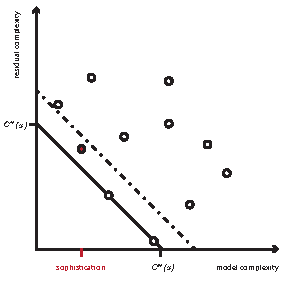
\includegraphics[width=\textwidth]{./img/sophistication.pdf}
  \end{minipage}
  \begin{minipage}{0.40\textwidth}
     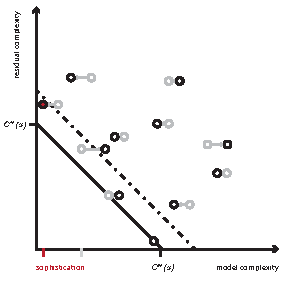
\includegraphics[width=\textwidth]{./img/sophistication-jump.pdf}
  \end{minipage}
  \caption{\small (left) Two-part representations of $x$ by the two components of their codelength. The Kolmogorov complexity $C^\M(x)$, appearing as a black diagonal, provides a lower bound on the total codelength. We consider only representations that are close to this optimum, with the threshold represented by a dashed line. The size of the smallest model below the threshold is the sophistication of the data. (right) The same image, after a constant perturbation in the model complexity caused by a change in numbering.}
  \label{fig:diagram}
\end{figure*}

A valid definition of $S$ must contend with two important issues. First, the details of the way the model is encoded are important. There are two technically distinct approaches; in one of these one has to deal with the so-called ``nickname problem'' that strangely remains unresolved in several publications. These definitions yield a sophistication that is highly dependent on the chosen programming language, unless special care is taken, as discussed in Section~\ref{section:indices}.

The second issue is that of striking the right balance between under- and overfitting, which we consider in Section~\ref{section:balance}. Overfitting is a common problem in statistics, that refers to the tendency to choose a complex model that provides a very good fit to the observed data, but does not generalise well to unseen data. In the case of sophistication, overfitting occurs if the model that determines the sophistication contains much or even all of the noise. In statistics, overfitting is often addressed by penalising complex models. In sophistication, however, such penalties tend to break the balance between structural information and noise, and lead to the opposite problem: underfitting.

Underfitting occurs when the selected model is simple, but fails to represent some of the structure present in the data. This is also a problem for sophistication because the models under consideration are so powerful. In particular, in any programming language, there are programs that implement an interpreter for \emph{another} language. Such \emph{universal models} are \emph{simple}, since they can be described with a relatively small number of bits, yet are able to represent the data using a code within a constant from the Kolmogorov complexity. Such a two-part representation essentially encodes all information as noise. If complex models are penalized, then the problem becomes to make sure that universal models are not \emph{always} preferred for complex data. The usual workaround is to restrict the set of allowed models, for instance to total functions. While this excludes universal models, it is questionable whether it adequately solves the problem of underfitting in general.

Finally, In the discussion in Section~\ref{section:conclusion} we argue that while two-part coding can yield useful insights into the structure of the data and allows us to identify some models as poor representations, it is probably not possible to uniquely separate structure from noise and identify a \emph{single} model as ``best'': in general many models, of vastly different complexities, may be reasonable representations. Rather than doggedly trying to ``fix'' this property of algorithmic statistics, we propose embracing the idea that the data allows for multiple equivalent interpretations of which information is structured, and which is random, and that there is no such thing as sophistication.

\enlargethispage{3\baselineskip} 
\section{Notation}
The following notation allows us to generalize across all definitions and variants, save the occasional exception which we will highlight individually.

Let $\B = \{0,1\}^*$. We deal with partial computable functions $f: \B \times \B \to \B$, which we will also call \emph{models}. A function is called \emph{prefix} if its domain, $\text{dom}_z(f)~=~\{y~:~f(y,~z)~\neq \infty\}$, is a prefix free set for all $z$, i.e. no string in $\text{dom}_z(f)$ is a prefix of another. A function $f$ is \emph{total} if $\forall_z \text{dom}_z(f) = \B$. In most cases, we do not use the second argument, and we adopt the convention that $f(x) = f(x, \epsilon)$.

A \emph{numbering} is an enumeration of of the partial computable functions, denoted as $\psi_1, \psi_2, \ldots$ or simply $\psi$. We fix one canonical effective numbering $\phi$. We call a numbering $\psi$ \emph{acceptable} if there exist total, computable functions $a, b: \N \to \N$ with $\forall: i$, $\phi_i = \psi_{b(i)}$ and  $\psi_i = \phi_{a(i)}$.

A \emph{model class} is a set of model indices. We distinguish four classes:
\begin{itemize} 
  \item The indices of the partial computable functions $\C=\N$.
  \item The total functions $\T=\{i:\tn{$\phi_i$ is total}\}$. Note that $\T$ is not computably enumerable.
  \item $\K$ is an enumerable set such that $\{\phi_i:i\in\K\}$ is the set of all partial computable prefix functions.
  \item The finite sets: $\F$ is an enumerable set such that $\{\phi_i:i\in\F\}$ contains a uniform code for every finite set.\footnote{A uniform code for a set $S$ is a surjective prefix function $f:\{0,1\}^{\lceil\log|S|\rceil}\to S$.}
\end{itemize}
A model class is thus defined in reference to a specific numbering, indicated by the context.

We sometimes need to map binary strings to a prefix-free set. We denote by $\br{x}$ the prefix-encoded representation for $x$. We require that the mapping satisfies $|\br{x}| = |x|+O(\log(|x|)$ (see eg. \cite[Section~1.4]{li1993introduction}). To simplify notation, we will sometimes conflate natural numbers and binary strings, implicitly using the ordering $(0, \epsilon)$, $(1, 0)$, $(2, 1)$, $(3, 00)$, $(4, 01)$, \ldots  

For technical reasons, we deviate slightly from the traditional notation of Kolmogorov complexity: we define the $\M$-Kolmogorov complexity of a binary string $x$, with respect to a model class $\M$ and a numbering $\psi$, as follows $C^{\M,\psi}(x\mid z)=\min\{\bar\imath y:\psi_i(y; z)=x,i\in\M\}$, with $C^{\M,\psi}(x) = C^{\M,\psi}(x\mid \epsilon)$. We may drop the numbering parameter when the distinction is not relevant. Under this notation $C^\C(x)$ corresponds to the plain Kolmogorov complexity $C(x)$ and $C^\K(x)$ corresponds to the prefix-free version $K(x)$. We can also represent the smallest two-part description of $x$ using a given model $\phi_i$ as $C^{\{i\}}(x)$. The complexity of a finite set is defined an the complexity of an explicit enumeration.

We use a choice of numbering for the purpose that is normally served by the universal Turing machine. The choice is a matter of taste: a UTM determines a numbering, and vice versa. The reason that we prefer to work with numberings is that it highlights an important issue: while Kolmogorov complexity is invariant to the choice of numbering this property does not immediately carry over to sophistication: for some treatments, the result is highly dependent on the chosen numbering (as shown in the next section). 
 
\section{Inefficient indices}
\label{section:indices}

The simplest approach to sophistication would be to `open up' the Kolmogorov complexity and to see which program on the universal Turing machine achieves the smallest description length: the program that \emph{witnesses} the Kolmogorov complexity. Since any UTM uses a two-part coding, its programs consist of a model and an input:

\begin{definition}[Index sophistication]
Let $\psi$ be an acceptable numbering. Let $\M$ be the model class from which candidates are chosen, and let $\Nm$ be the model class that determines the minimum achievable complexity. Let $c$ be a fixed constant. The \emph{index sophistication} is:
\[
\s_{\text{index}}^{\M,\Nm,\psi,c}(x) = \min\left\{ |i| : i \in \M, C^{\{i\}, \psi}(x) \leq C^{\Nm, \psi}(x)+c   \right\} \p
\]
When $\M = \Nm$, we will abbreviate with $\s^{\Nm,\psi,c}$. \label{definition:index}
\end{definition}
Koppel and Atlan's treatment \cite{koppelSoph1988,koppel1991almost}, where the name \emph{sophistication} originates, follows this basic logic, although it contains idiosyncracies like the use of monotonic models, and an extension to infinite strings. As the subsequent history of sophistication has discarded these, we will not discuss them here.

In \cite{antunes2009sophistication,antunes2013sophistication} Koppel's principle is limited to finite strings, with the total functions as a model class. The definition used is similar to $s_\text{index}^{\T, \C,\psi,c}$, with one exception: the total complexity of a witness $(i,y)$ is measured as $|i|+|y|$ without the cost of delimiting the two. This difference is not relevant to the point we make in this section. The restriction to total classes is a common approach, perhaps used because it helps to avoid underfitting, which we will discuss in the next section. 

\begin{lemma}
Let $\s^\psi$ denote any index sophistication with respect to numbering $\psi$.
There are acceptable numberings $\psi$ and $\xi$ such that for all $x$:\\
\-\hspace{2.8em} $|\s^\psi(x) - \s^\xi(x)|\geq \tfrac{1}{2}\min\{\s^\psi(x),\s^\xi(x)\}$.
\end{lemma}
\begin{proof}
Let $s_i$ be the string consisting of $2^{i}$ zeroes followed by a one. Define $\psi, \xi$ such that $\psi_j(x) = \phi_i(x)$ for $j = s_{2i}$ and $\xi_j(x) = \phi_i(x)$ for $j = s_{2i+1}$, with all other functions returning $\infty$ for all inputs. Choose any $x$ and assume w.l.o.g. that $\s^\psi(x)\le s^\xi(x)$. By construction, we have $2\s^\psi(x)  \leq \s^\xi(x)$.
\end{proof}
Thus, the length of the index is a very poor indicator of model complexity. For a robust measure, define the complexity of functions as in \cite{grunwald2004shannon,vitanyi2004meaningful} by $C^{\M,\psi}(f) = \min\{C^{\M,\psi}(i):\phi_i=f\}$.
Lemma~\ref{lemma:invariance} in the appendix shows that $C^\C(f)$ and $C^\K(f)$ are invariant: they are objective properties of a function.

Note that such perversely inefficient numberings are not an issue for Kolmogorov complexity. If our UTM uses an inefficient numbering, we can switch to a more efficient one at only a constant cost, keeping the complexity the same, up to a constant. For sophistication, however the choice of numbering is crucial.

There are two ways to use the model complexity $C^\M(\phi_i)$ for more robust attempts to define sophistication. Confusingly, both are used in the literature. First, we can measure the complexity of the \emph{model} using $C^{\M,\psi}(\phi_i)$, which is then the size of the first part of a two-part code describing the data. For instance, this approach is used in  \cite{cover1985kolmogorov,gacs2001algorithmic,vitanyi2004meaningful,gellmann1996information} and in most of the present paper.

Second, we can stick to using the length of the index as the measure of sophistication, but restrict the allowed numberings. This approach is taken by Adriaans in \cite{adriaans2012facticity}, which defines \emph{facticity} as $\s_\text{index}^{\C,\psi,0}$, but only allows numberings that are \emph{faithful}: $\forall i \exists j : \psi_i=\psi_j, |j|\le C^{\C}(\psi_j)+c$, for some constant $c$.

We prove in the appendix that---contrary to Adriaans' suggestion---there actually do exist faithful, acceptable numberings (Lemma~\ref{lemma:faithful-numberings}). However even choosing a faithful index is not quite enough. The Kolmogorov complexity uses representations of the form $\bar\imath y$, where the bar denotes some straightforward prefix encoding to delimit the model description $i$ from its input $y$. If we define a second prefix encoding $\tilde{\imath}$, with $|\bar\imath|-|\tilde\imath|$ unbounded, we can define a second representation $\bar u \tilde \imath y$, at a constant overhead $|\br{u}|$, and gain more than $|\br{u}|$ for sufficiently complex strings, resulting in a bounded sophistication.

We continue with a sophistication that avoids these issues. Let $C'^{\M, \psi} = C^\K(\psi_i) + min\{|y| : \psi_i(y) = x\}$. We define sophistication as:

\begin{definition}[Sophistication]
\[
\s^{\M,\Nm,\psi,c}(x)=\min\left\{C^\K(\phi_i):i\in\M,C'^{\{i\},\psi}(x)\le C^{\Nm,\psi}(x)+c\right\}.
\]
\end{definition}

\section{Balancing under- and overfitting}
\label{section:balance}

In the previous section, we saw the first glimpse of the delicate balance between the two code components in sophistication. We will investigate this balance, starting with the variant $\s^{\K,\psi,c}$. This variant itself is not used anywhere in the literature, but it helps to illustrate the issues we wish to discuss.

$\K$ has representations with all information except a constant in the input and representations with all information in the model. The downside to this balance is that it becomes easy to show a lack of invariance: by tweaking the numbering so that models in a specific subset $\M'\subset\M$ become cheaper to represent by an arbitrary amount relative to others, so that a model in $\M'$ always determines the sophistication.

This means that for model classes with a universal model, we can choose our numbering to make $S^\K$ either bounded, or equal to the complexity:

\begin{theorem}[Underfitting]
Let $\M$ be a model class containing a universal model $\phi_u$, with the property that $\exists c \forall i \in \M, x : C'^{\{u\}}(x) \leq C'^{\{i\}}(x) + c$. Then, for some numberings $\s^{\M,\psi,c}$ is bounded. \label{theorem:underfitting}
\end{theorem}

This result is well known and many treatments avoid it by restricting the model class. Less well known is perhaps that the same holds in the other direction: for some numberings the singletons always determine the sophistication. 

\begin{theorem}[Overfitting]
Let $\M \subseteq \K$ be a model class where for every $x\in\X$ there is a singleton model $i\in\M$ with $\phi_i(\epsilon)=x$. Then there is a numbering $\psi$, and a constant $c$, such that for all $x\in\X$ we have $C^\M(x)-S^{\M,\psi,c}(x)\leq c$.\label{theorem:overfitting}
\end{theorem}
The proofs of both theorems rely on a simple principle: for certain $\M' \subset \M$, there exist numberings which have the effect of penalizing $C^\K(\phi_i)$ for any model outside $\M'$ by an arbitrary constant amount. We can use this to effectively `push' these models outside of the range of candidates, ensuring that, under this numbering, a model in $\M'$ always determines the sophistication.

For these theorems, this means setting $\M' = \{u\}$, with $\phi_u$ a universal model, or letting $\M'$ be the singletons. The requirements for $\M'$ are strict, and slightly complex. The following lemma gives a set of sufficient conditions.

\begin{restatable}{lemma}{coolone}
\label{lemma:thecoolone}
  Let $\M$ be any model class, let $\X$ be any set of binary strings and let $D:\B\to\N$ be a computable decoding function with a prefix-free domain that maps function descriptions to their indices in $\phi$. Let $\M'= \tn{range}(D)$. Further assume there is a constant $c$ such that:\\
\-\hspace{1cm}(1) $\forall_{m\in\M'}:\min\{|p|:\phi_{D(p)}=\phi_m\}\le C^{\K,\phi}(\phi_m)+c$\\
\-\hspace{1cm}(2) $\forall_{x\in\X}:C'^{\M',\phi}(x)-C'^{\M,\phi}(x)\le c$.\\
Then there is an enumeration $\psi$ of the partial recursive functions such that $S^{\M,\psi,c}(x) = |\br{0}|+S^{\M',\phi,c}(x)$ for all $x\in\X$.
\end{restatable}

\begin{proof}
We define the numbering $\psi$ as follows:
\[
\psi_0(p) = 1^r 0 D(p), \;\;\;
\psi_{1^r0i}(p) = \phi_i(p), \;\;\;
\psi_j(\cdot) = \infty \;\text{if $j$ contains no zeroes.}
\]
We will show that under the $\psi$, the best representation for $x$ with $m\in\M'$ is always better than the best using some $m\notin\M'$. First suppose $m\in\M'$. Then
\begin{align*}
   C^{\K,\psi}(\phi_m) &=\min\{|\bar\jmath q|:\psi_{\psi_j(q)}=\phi_m\} \leq\min\{|\bar0 q|:\psi_{\psi_0(q)}=\phi_mm\} \\ 
   &=\min\{|\bar0 q|:\psi_{1^r0 D(q)}=\phi_m\} =\min\{|q|:\phi_{D(q)}=\phi_m\} + |\bar 0|\\
   &\leq C^{\K,\phi}(\phi_m)+c+|\br{0}|,
\end{align*}
where the last inequality uses assumption (1).

Now assume that the best model $m$ for $x$ is not in $\M'$. 
Let $i$ be the index of $m$ with the shortest description, i.e. it achieves the minimum in $C^{\K, \psi}(\phi_m)=\min\left\{C^{\K,\psi}(i):\psi_i=\phi_m\right\}$.
There are two possibilities. Either $i = 0$, in which case we have $C^{\K,\psi}(m)\ge r$ because $\phi_0$ cannot output zero and all other $\psi$-programs are at least $r$ bits long. Otherwise, we can bound
\begin{align*}
C^{\K,\psi}(\phi_m)&=C^{\K,\psi}(m)=C^{\K,\psi}(1^r0j)\\
&\ge C^{\K,\psi}(j)-c' \ge C^{\K,\phi}(j)+r+1-c'\\
&=C^{\K,\phi}(m)+r+1-c'.
\end{align*}
Now choose $r=c''+\max\left\{C^{\K,\psi}(\phi_0),c'-1\right\}$. Then substitution yields, for both cases, 
$C^{\K,\phi}(m)\ge c''+C^{\K,\psi}(m)$. Combining the inequalities above, for any model $\phi_g$ with $g\not\in\M'$, there is a model $\phi_f$ with$f\in\M$ such that
\[\begin{split}
C^{\K,\psi}(\phi_g)+&\min \{|y| : \phi_g(y) = x\} \ge C^{\K,^\phi}(\phi_g)+\min\{|y| : \phi_g(y) = x\}+c''\\
&\ge C^{\K,\psi}(\phi_f)+\min \{|y| : \phi_f(y) = x\} -2c+c'' -|\bar0|.
\end{split}\]
A sufficiently large $c''$ ensures the best representation is in $\M'$ for all $x\in\X$.
\end{proof}

Theorems~\ref{theorem:underfitting} and \ref{theorem:overfitting} follow as corollaries. For Theorem~\ref{theorem:underfitting}:
\begin{proof}
Let $D$ be a prefix function as in Lemma~\ref{lemma:thecoolone} such that it returns the index of $u$ for the argument $\epsilon$ and $\infty$ for any other argument. That is, $\M' = \{u\}$. This construction satisfies the conditions 1 and 2 from Lemma~\ref{lemma:thecoolone}; invoking it we find that there exists an acceptable numbering $\psi$ for which $\s^{\M,\psi}(x) = \s^{\M', \phi, c}(x) + c$. Since $\M'$ contains only a single model, $\s^{\M',\phi, c}(x)$ is constant.
\end{proof}

And for Theorem~\ref{theorem:overfitting}:

\begin{proof}
Let $\phi_i$ be a singleton for $x$ as described. Note that since $\phi_i$ is a prefix function, since $\phi_i$ is defined for input $\epsilon$ then it cannot be defined for any other input. Pick $i,x$ with $\phi_i(\epsilon)=x$. Note that $x$ can be computed from $i$ and a fixed program, so there is a $c$ such that $C^{\K, \phi}(x)\le C^{\K, \phi}(\phi_i)+c$. Vice versa, given any $x$ we can construct an index of $\phi_i$, since $\phi$ is an acceptable numbering. Therefore $|C^{\K,\phi}(\phi_i)-C^{\K, \phi}(x)|\le c$.

We now define a computable function $D$ by $D(\bar\imath y)=j$ where $\psi_j(\epsilon) = \phi_i(y)$.  We will show that the two conditions of Lemma~\ref{lemma:thecoolone} hold for the prefix function $D$.

(1) Let $f$ be any function in the range of $D$, and $x$ its output. Then $\min\{|p|:\psi_{D(p)}=f\}=\min\{|\bar\imath q|:\phi_i(q)=x\}=C^{\K}(x) \le C^{\K}(f)+c$. (2) On the one hand $C^{\M',\psi}(x)\le C^\K(f)+|\epsilon|\le C^\K(x)+c$. On the other hand, $C^{\M,\psi}(x)$ is an effective description of $x$, so $C^{\K}(x)$ is at most a constant larger. Together, these inequalities establish the second condition.

Now, by Lemma~\ref{lemma:thecoolone} there is a numbering $\psi_1,\psi_2,\ldots$ such that $\s^{\M,\phi}(x)=|\bar 0|+S^{\M',\psi}(x)$. We observed that $|C^{\K}(f)-C^{\K}(x)|\le c_0$ for any $f\in\M'$, so $\s^{\M',\psi, c}(x)\ge C^{\K}(x)-c_0$. This proves the lemma.
\end{proof}

\noindent Thus, in this balanced sophistication, there is no invariance: all information can be seen as structure, or as noise, depending on the numbering. To avoid these issues, existing proposals upset the balance to exclude or penalize the universal models, and possibly the singleton models. 

\subsection{Overfitting}

We will now review the treatments in the literature that show overfitting. The first is the structure function, proposed by Kolmogorov: most likely the first attempt at separating structure from noise in an objective manner. Kolmogorov defined the function
\[
h_x(\alpha) = \min \left \{\log |S| : S \ni x, C^\K(s) \leq \alpha \right \} 
\]
and suggested that the smallest set for which $C^\K(S) + \log|S| \leq C^\K(S) + c$ for some pre-chosen constant $c$ can be seen as capturing all the structure in $x$ \cite{cover1985kolmogorov}. This is equivalent to the sophistication $\s^{\F,\K,\psi,c}$. Theorem~\ref{theorem:overfitting} shows  there are numberings for which this sophistication is always equal to $C^\K(x)$. Thus, either this is true for all numberings, or this sophistication is not invariant. 
 
In \cite{gacs2001algorithmic} the idea of the structure function is extended to the notion of an \emph{algorithmic sufficient statistic}. This is essentially the witness to the sophistication $\s^{\F,\K,\psi,c}(x)$. Thus, by Lemma~\ref{theorem:overfitting}, there exist numberings such that for all $x$, $\{x\}$ is the minimal sufficient statistic. 

It may be argued that the slack parameter $c$ in the sophistication, which determines the allowed gap between a candidate representation and the complexity, should be allowed to depend on the numbering, but this dependence has not been mentioned in the literature and there is no clear way to determine how this constant should be chosen on the basis of a given numbering. 

In traditional statistics, overfitting is often addressed by imposing a penalty on complex models. As we have seen, a strong penalty, such as the one imposed by an inefficient prefix encoding of the model, will immediately cause underfitting. A more subtle approach is to allow descriptions that are not self delimiting. The gap between self-delimiting and non self-delimiting descriptions grows without bound 
\cite[Section~4.5.5]{li1993introduction}, so that for sufficiently complex inputs, some information will have to be placed in the noise part of the code, since placing all information in the model results in a self-delimiting description. This eliminates the singletons as viable candidates. This approach is taken by Vit\'anyi \cite{vitanyi2004meaningful} and by Adriaans \cite{adriaans2012facticity}. Such measures thus help reduce the overfitting problem, but they only increase the tendency to underfit. We also pay the price that the models can no longer be equated with probability measures, weakening the link to traditional statistics and probability theory.

\subsection{Underfitting}
\label{section:underfitting}

The existence of universal models is a widely acknowledged problem for sophistication, and most proposals avoid it by limiting the class of allowed models to exclude them. It is known that there are strings for which $\s^{F, K, \psi, c}$, $\s^{T, \psi, c}$, $\s^{T, \K, \psi, c}$ are close to the length of the string (up to a logarithmic term). These are the so-called absolutely non-stochastic strings \cite{shen1983concept}. Proofs for the sophistications mentioned can be found in \cite{gacs2001algorithmic}, \cite{antunes2009sophistication} and \cite{vitanyi2004meaningful} respectively. The existence of these strings is independent of the numbering chosen. 

However, the problem of the singletons remains. Only one model class eliminates both the singletons and the universal model: $\T$. The only proposal we are aware of that uses an efficient model representation \emph{and} excludes the universal models \emph{and} excludes the singletons is \cite{vitanyi2004meaningful}, where $\s^{\T,\K,\psi,c}$ is used. While this invalidates straightforward proofs of boundedness, there is no evidence that $S^{\T,\K,\psi, c}(x)$ is actually invariant either.

While under $S^{\T,\K,\psi, c}(x)$ there are strings with high sophistication, these may not conform to sophistication's motivating intuition. To show this, we need the concept of depth:

\begin{definition}[Depth\cite{bennett1988logical,antunes2006computational}]\belowdisplayskip=-12pt
Let $U$ be some universal Turing machine, so that $U(\bar\imath y) = \phi_i(y)$. Let $U^t$ be a simulation of this machine, which is allowed to run for at most $t$ steps, and returns $0$ if it has not yet finished at that point. Let $C^\M_t(x) = \min\{|\bar\imath y| : U^t(\bar\imath y) = x, \phi_i \in \M\}$. The \emph{$c$-depth} is $d^{\M,c}(x) = \min \left\{t : C^\M_t(x) - C^\M(x) \leq c \right\}$.
\end{definition}
Deep strings are those that can only be optimally compressed with a great investment of time. We note that it is exceedingly unlikely that a deep string is sampled from a shallow distribution \cite{bloem2014safe,bennett1988logical}. 
 
\begin{theorem}
Let $A(n)$ be the single-argument Ackermann function and $c$ some arbitrary constant. There are numberings such that for strings with depth $d^{\C,c}(x) \leq A(C^\C(x))$ the sophistication $\s^{\T, \K, \psi, c}$ is bounded.\label{thm:depth}
\end{theorem}

\begin{proof}
Let $U(\bar\imath y)$ be some universal Turing machine, and let $U^A(\bar\imath y)$ be a simulation of that machine which outputs $0$ if the number of steps taken exceeds $A(|\bar\imath y|)$. Let $u$ be the index of the function $U^A$ in the standard enumeration.

Let $D$ be a prefix function with $D(\epsilon) = u$. We can instantiate Lemma~\ref{lemma:thecoolone} with $D$, $\M' = \{\phi_u\}$ and $X = \{x : d^{\C,c}(x) \leq A(C(x))\}$. This tells us that there exists a numbering for which $\s^{\T, \K,\psi,c}(x) = \s^{\M', \psi, c}(x) + |\bar0| \leq c$ for all $x \in X$.
\end{proof}

\noindent This shows that while high-sophistication strings exist, they do not behave as expected. Consider a string that is typical for a shallow model, say some elaborate probabilistic automaton. Under $\s^{\T,\K, \psi,c}$, no matter how high the complexity of the automaton, the sophistication is bounded. We could encode the collected works of Shakespeare in its transition graph, and this information would be counted as noise by the sophistication. Any structure simple enough to be exploited within the time bound of the Ackermann function will not be seen as `meaningful information'. Only structure so deep that it would take beyond the lifetime of the universe to decompress would count towards sophistication. In the remainder we will refer to strings $x$ with $d^{\C,c}(x) \leq A(C(x))$ as \emph{non-deep} strings.

The relation between $S(x)$ and $d(x)$ is also investigated in \cite{antunes2013sophistication}, where it is shown that within a logarithmic error term on the sophistication and the slack, they are identical. Our point is not the similarity between the two, but that for all practical strings, the sophistication is bounded. This contradicts the intuition that sophistication measures structure, as it seems to suggest that all strings we can possibly hope to understand or generate contain no structure, save a constant amount. The alternative is that under other numberings these strings \emph{would} have structure, but then the sophistication would no longer be invariant.

As for the strings with high sophistication, they have the property that they can be compressed far better with partial functions than with total: they are non-typical for the model class $\T$. This suggests that the `non-stochastic' property of strings with high sophistication \cite{shen1983concept,vereshchagin2004kolmogorov} says more about depth and totality than it does about structure and noise.

\subsection{Other variants}
\label{section:other}

By moving away from the idea of two-part coding, the mechanics of lemma~\ref{lemma:thecoolone} can be avoided. In \cite{mota2013sophistication}, the \emph{naive sophistication} is introduced. We will define a generic version, parametrized by model class. 

\begin{definition}[Naive sophistication]
Let $C_i(x) = \min\left\{|y| : \phi_i(y) = x\right\}$. Then we define the \emph{naive sophistication} as:
\[
\s_\text{naive}^{\M, \psi, c}(x) = \min\left\{C^\K(\psi_i) : i \in \M, C_i(x) - C^\K(x\mid s) \leq c \right\} \p
\]
\end{definition} 

The condition now is not that the two-part code length corresponds to the Kolmogorov complexity, as in the regular sophistication, but that the \emph{randomness deficiency} is less than a constant. $\s_\text{naive}^{\F,\psi,c}(x)$ corresponds to the version in \cite{mota2013sophistication}. The switch to the randomness deficiency avoids Theorem~\ref{theorem:overfitting}, but we end up with the same problem as Vit\'anyi's sophistication (Theorem~\ref{thm:depth}): for non-deep strings $s^{\T, \psi, c}$ is defined by the model $U^A$, and thus bounded.

We cannot show that $s^{\F, \psi, c}(x)$ is bounded for non-deep strings, but this is only a consequence of the use of sets, not of the switch to randomness deficiency as a condition. \emph{Any} set sophistication is necessarily lower-bounded by the function $\text{set}(x) = \min\left\{C^\K(S) : x \in S\right\}$ and if this function were bounded, it would suggest that a finite amount of sets contained all strings.
\begin{theorem}
Let $x$ be a non-deep string. Then $\s_\text{naive}^{\T,\K,\psi,c}(x)$ is bounded and
\[
\text{set}(x) \leq \s_\text{naive}^{\F,\K,\psi,c}(x) \leq C^\K(C^\K(x)) \p
\]\label{theorem:naive}
\end{theorem}
\begin{proof}
For the first part, we take the model $U^A$ as defined in Section~\ref{section:underfitting}.For some numbering $\psi$, we have $C_i(x) - C^\K(x\mid S) \leq 0$, thus $\s_\text{naive}^{\T,\psi,c}(x) \leq C^K(U^A)$. 
For the second part, let $C^\K(x) = k$ and $S^A_k = \{x \mid \exists p : U^A(p) = x, |p| \leq k\}$, and let $S_k = \{x : \exists p : U(p) = x, |p| \leq k\}$. We will first show that $C^\K(x) = C^\K(S_k^A) + \log |S_k^A|$ up to a constant., ie $S^A_k$ is \emph{optimal} for $x$. It's known that  $\log |S^A_k| \leq \log |S_k| = k - K(k) + O(1)$ \cite{gacs2001algorithmic}. We also have $C^\K(S_k^A) \leq C^\K(k) + O(1)$. Thus
\begin{align*} 
C^\K(x) &= k + C^\K(k) -C^\K(k) \\
&\geq C^\K(S^k) + \log |S^A_k| \geq C^\K(x) \\  
\end{align*}
Where all (in)equalities are up to a constant. The last inequality follows from the fact that $C^\K(x)$ is the smallest possible self-delimiting description. By Lemma III.9 in \cite{gacs2001algorithmic}, optimality implies typicality, so the randomness deficiency of $x$ in $S_k^A$ is bounded. Thus, for large enough $c$, $\s_\text{naive}^{\F,\psi,c}(x) \leq C^\K(C^\K(k))$.
\end{proof}
Another approach is the \emph{coarse sophistication} \cite{antunes2009sophistication}. The simplest definition comes from \cite{mota2013sophistication}:
\[
\s^{\M,\Nm,\psi, c}_\text{coarse}(x) = \min_c\left\{\s^{\M,\Nm,\psi,c}(x) + c \right\} \p
\]
Again, this variant avoids the pitfalls of Theorem~\ref{theorem:overfitting}. If a set of $x$s has witnesses $S_x$ that are as good as the singleton set, up to a constant, but with smaller $C^\K(S)$ by more than a constant, the added penalty $c$ will eventually be much less than the gain for the simpler witness, and the singletons will not determine the coarse sophistication. It was noted in \cite{antunes2009sophistication} that the coarse sophistication is within a logarithmic term of the busy beaver depth, again relating sophistication to depth. For our purposes we can show that, as with the naive sophistication the total function version is bounded and the set version grows very slowly:
\begin{theorem}
Let $c_0$ be some constant. Then for all non-deep strings $x$ we have that $\s_\text{coarse}^{\T,\K,\psi,c}(x)$ is bounded and
\[
\text{set}(x) \leq s_\text{coarse}^{\F,\K,\psi,c}(x) \leq C^\K(C^\K(x)) + c_0
\].\label{theorem:coarse}
\end{theorem}
\begin{proof}
For $\s_\text{coarse}^{\T,\K,\psi,c}(x)$, again take $U^A$ as a model. By Lemma~\ref{lemma:thecoolone}, there exists a numbering $\psi$ so that for all shallow $x$, a representation with $U^A$ witnesses the Kolmogorov complexity exactly. Thus $\s_\text{coarse}^{\T,\K,\psi,c}(x) \leq C^\K(U^A)$ for all non-deep strings.
For the set case, we re-use $S_k^A$ as defined in the proof of Theorem~\ref{theorem:naive}. If we set $c$ to $C^\K(C^\K(x))$ in the regular sophistication, the upper bound follows. The lower bound follows as established earlier.
\end{proof}
In \cite{vereshchagin2013algorithmic}, Vereshchagin proposes a strongly algorithmic sufficient statistic. Whereas the regular algorithmic sufficient statistic $S$ from \cite{gacs2001algorithmic} has as one of its requirement that $C^\K(S\mid x)$ is constant, the strong variant imposes the requirement that $C^\T(S\mid x)$ is also constant. This reduces the problems of underfitting discussed in this section, but since $C^\T(\{x\}\mid x)$ is bounded, by Theorem~\ref{theorem:overfitting}, overfitting remains a problem: for a given constant deviation allowed from the Kolmogorov complexity, there exist numberings so that only the singletons come within that constant.

Finally, we must mention \emph{effective complexity} \cite{gellmann1996information}, proposed by Gell-Man and Lloyd. This measure is unique, in that it was formulated from the perspective of physics. Nevertheless, it fits the mold of sophistication very neatly. The models used are computable probability distributions on finite sets, and all candidates that come within a constant of the Kolmogorov complexity are considered. The complexity of the model is correctly measured by its Kolmogorov complexity. We note that this means that Lemma~\ref{theorem:overfitting} applies. Unlike other sophistication measures, here it is not the smallest model which is chosen, but the one which reproduces the data with in the shortest time. Thus, if there are multiple candidates, this approach would likely favor the singleton sets. In \cite{gell2004nonextensive}, the authors abandon this approach, and note the choice from the set of candidates is a subjective one, which depends on context.

\section{Discussion and conclusion}
\label{section:conclusion} 

We have criticized existing measures of sophistication and shown technical problems with all of them. But that does not in itself mean that it should be impossible to come up with a sound measure. The intuition throughout the literature, starting with the structure function, appears to be that the crucial property is whether a string is typical for a model, and that this typicality can be tested: another random choice from that model should select a string with the same structure. This idea is bold, but not necessarily unreasonable. Nevertheless, in this section we offer the opinion that such a clean-cut separation \emph{cannot} be made to work. We provide two arguments to support this belief.

For the first argument, we take a generative perspective. We can generate data from a model $\phi_i, i \in \K$, by feeding it random bits until it produces an output. We will call the resulting probability distribution $p_i(x) = \sum_{y:\phi_i(y) = x} 2^{-|y|}$. In this setting, a sophistication could be called \emph{consistent} if, for data of sufficiently high Kolmogorov complexity, it reflects the complexity of that distribution from which it originated. Suppose the data is sampled from the universal distribution: let $\phi_u(\bar\imath y)=\phi_i(y)$ and sample from $p_u$ as described above. Then the initial bits will determine the prefix encoded index $\bar\imath$ of the function $\phi_i$ that $\phi_u$ will subsequently emulate, and the remaining bits are used as inputs to $\phi_i$. We now ask, what should be the sophistication of the resulting data? 
\enlargethispage{3\baselineskip}
 
Certainly, if we have to judge based only on the data, we cannot exclude the possibility that the data was sampled from $p_u$: after all, it was.  On the other hand, neither can we exclude the possibility that it came from $p_i$, as again, it did! It seems unjustified to assume that, based on only the data, all but one model can always be disqualified.

Consider the following metaphor. We are given a a bitmap image of the painting \emph{Impression of a Sunrise}. There are many good models for this string, from very generic to very specific. Sophistication suggests that we can choose one of these as the objective, intrinsic model of the data. The universal model says that it is `some compressible, finite object'. Another might say that it is `an image'. Even more specific would be `a painting', `a Monet', or specifically `the painting \emph{Impression of a Sunrise}'. A sound sophistication should be able to select one of these as the proper representation of structure in the data, and disqualify the others as over- or underfitting. But how should we be able to say that the data is intrinsically more of a painting than an image? More of a Monet than a painting? Intuitively, such distinctions require further assumptions, or a second sample from the same distribution.

The second reason we believe sophistication will elude definition is more technical. Given an input $x$ and some model class, say $\C$, consider the set of all possible two-part representations of $x$. Now, when the numbering is changed, the codelength of the model part of all these representations will change. This is illustrated in the right graph in Figure~\ref{fig:diagram}. The invariance theorem expresses that this change is limited by a constant term that does not depend on $x$. So for sufficiently large $x$, the horizontal shift of all the representations will be relatively small. However, even this small shift can push some representations out of the acceptable region (indicated by the dashed line), and pull others in. This may lead to a different representation determining the sophistication, one whose \emph{total} codelength is close to what it was before, but whose \emph{model} codelength can be anywhere between $0$ and $C^\C(x)$. If such jumps can occur, the sophistication is not invariant. And while we cannot \emph{prove} in general that such jumps can always occur, there seems to be no reason to believe that they do not. Indeed, in \cite{antunes2013sophistication} it is shown that logarithmic changes in the slack parameter can cause these effects.

So we take a skeptical view of sophistication. Note that part of the theory is fine: there is nothing wrong with evaluating models for the data by comparing their two-part code lengths. In fact, the randomness deficiency $\delta(\phi_i,x)=-\log p_i(x)-C^\K(x\mid i)$ of a model $\phi_i$ has a direct statistical interpretation as a measure of counterevidence against the hypothesis that it generated the data---if $p_i$ truly generated the data, then the probability that the randomness deficiency is more than $k$ bits is less than $2^{-k}$ \cite[Lemma~6]{bloem2014safe}. In the Monet example above, this will allow us to disqualify the model expressing that the data is actually, say, a recording of jazz music.

But fundamental problems arise as soon as a hard cut-off is introduced on how far we are allowed to deviate from the minimum determined by the Kolmogorov complexity. In our opinion, a lot of measures taken in the literature to address problems with sophistication, such as restricting the model class or introducing model penalties, complicate the method and make problems harder to analyse, without actually addressing the fundamental issue. This is dangerous: if such ad-hoc fixes result in a theory that is hard to prove either wrong or right, it creates an artificial dead end for a valuable area of research. When the hard cut-off on which models are considered is avoided, on the other hand, all such measures are suddenly no longer necessary. What remains is a simple and elegant theory that can be used to sift through all possible models, disproving most while retaining a select number of interesting candidates for our further consideration.

\subsubsection*{\ackname}
\ldots
\hide{This publication was supported by the Dutch national program COMMIT and by  the Netherlands eScience center. We thank Tom Sterkenburg for interesting discussions.}

\bibliographystyle{plain}
\bibliography{facticity}

\appendix
\section{Appendix}
\begin{lemma}[Invariance of function complexity]
Let $\psi$ and $\eta$ be any two acceptable numberings. There exists a constant $c$ such that $\left| C^{\K,\psi}(f) - C^{\K, \eta}(f)\right | \leq c$ for all $f \in \C$ and $\left| C^{\C,\psi}(f) - C^{\C, \eta}(f)\right | \leq c$ for all $f \in \C$. \label{lemma:invariance}
\end{lemma}
\begin{proof}
Let $g(i)$ be the function such that $\psi_i=\eta_{g(i)}$.
\begin{align*}
C^{\C,\psi}&(f) = \min\left\{ C^{\C,\psi}(i) : \psi_i= f\right\} 
\geq \min\left\{ C^{\C, \eta}(i) : \psi_i= f\right\} - c\\
&= \min\left\{ C^{\C, \eta}(i) : \eta_{g(i)}= f\right\} - c
\geq \min\left\{ C^{\C, \eta}(i) : \eta_i= f\right\} - c' = C^{\C, \eta}(f).
\end{align*}
Reversing $\psi$ and $\eta$ for the opposite inequality. The same proof holds for $\K$.
\end{proof}
This lemma shows that the complexity of a function does not depend on the choice of
enumeration by more than a constant term.
%\enlargethispage{2\baselineskip} 

\begin{restatable}{lemma}{faithful}\label{lemma:faithful-numberings}
  There are faithful acceptable numberings.
\end{restatable}

\begin{proof}
Let $d \in \N$ be an index such that $\phi_d(y)=\infty$ for all $y$. Define
  \[\psi_q=\begin{cases}
    \phi_{\phi_i(p)}&\tn{if $q$ can be written as $\bar\imath p$ and $\phi_i(p)<\infty$,}\\
    \phi_d&\tn{otherwise.}\end{cases}
  \]
  To show that $\psi$ is faithful, pick any function $f$. Then
\[\begin{split}
C^{\C, \phi}(f)&=\min\{C^{\C, \phi}(i):\phi_i=f\} =\min\{\min\{|\bar a b|:\phi_a(b)=i\}:\phi_i=f\} \\
& =\min\{|\bar a b|:\phi_{\phi_a(b)}=f\}
 =\min\{|\bar a b|:\psi_{\bar a b}=f\}.
\end{split}\]
This shows there is a sufficiently small $\psi$ index.

To show that $\psi$ is acceptable, let $\phi_j$ denote the identity
function. Then a $\phi$-index $i$ can be mapped to a $\psi$-index
using the computable function $r(i)=\bar\jmath i$, so that
$\psi_{r(i)}(y)=\psi_{\bar\jmath i}(y)=\phi_i(y)$. For the reverse,
define $\phi_v(\bar\imath p, y)=\phi_{\phi_i(p)}(y)$. For fixed
$\bar\imath p$, the 
$s^n_m$-theorem \cite{kleene193notation} states that we can compute the $h$
such that $\phi_h(y)=\phi_v(\bar\imath p,y)$. Let $h(\bar\imath p)$
denote this index as a function of the program; further define
$h(q)=d$ if $q$ cannot be expressed as $\bar\imath p$. By
construction $h$ is total and computable. To check that the mapping
returns the correct function, rewrite $\phi_{h(\bar\imath
  p)}(y)=\phi_v(\bar\imath p,y)=\phi_{\phi_i(p)}(y)=\psi_{\bar\imath p}(y)$.
\end{proof}

\end{document}
